\documentclass[border=8pt, multi, tikz]{standalone}
%\usepackage{blocks}
\usepackage{import}
\subimport{layers/}{init}
\usetikzlibrary{positioning}

\def\ConvColor{rgb:yellow,5;red,2.5;white,5}
\def\ConvReluColor{rgb:yellow,5;red,5;white,5}
\def\PoolColor{rgb:red,1;black,0.3}
\def\UnpoolColor{rgb:blue,2;green,1;black,0.3}
\def\FcColor{rgb:blue,5;red,2.5;white,5}
\def\FcReluColor{rgb:blue,5;red,5;white,4}
\def\SoftmaxColor{rgb:magenta,5;black,7}


\newcommand{\copymidarrow}{\tikz \draw[-Stealth,line width =0.8mm,draw={rgb:blue,4;red,1;green,1;black,3}] (-0.3,0) -- ++(0.3,0);}

\begin{document}
	\begin{tikzpicture}
		\tikzstyle{connection}=[ultra thick,every node/.style={sloped,allow upside down},draw=\edgecolor,opacity=0.7]
		\tikzstyle{copyconnection}=[ultra thick,every node/.style={sloped,allow upside down},draw={rgb:blue,4;red,1;green,1;black,3},opacity=0.7]
		
		\node[canvas is zy plane at x=0] (temp) at (-5,0,0) {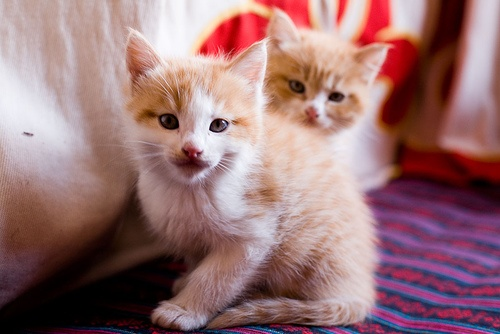
\includegraphics[width=6cm,height=6cm]{cats.jpg}};
		
		%%%%%%%%%%%%%%%%%%%%%%%%%%%%%%%%%%%%%%%%%%%%%%%%%%%%%%%%%%%%%%%%%%%%%%%%%%%%%%%%%%%%%%%%
		%% Draw Encoder
		%%%%%%%%%%%%%%%%%%%%%%%%%%%%%%%%%%%%%%%%%%%%%%%%%%%%%%%%%%%%%%%%%%%%%%%%%%%%%%%%%%%%%%%%
		% conv1_1,conv1_2
		\pic[shift={(0,0,0)}] at (0,0,0) {RightBandedBox={name=cr1,%
				xlabel={{"64","64"}},zlabel=I,fill=\ConvColor,bandfill=\ConvReluColor,%
				height=40,width={2,2},depth=40}};
		%pool1
		\pic[shift={(0,0,0)}] at (cr1-east) {Box={name=p1,%
				fill=\PoolColor,opacity=0.5,height=32,width=1,depth=32}};
		%%%%%%%%%%
		% conv2_1,conv2_2
		\pic[shift={(1,0,0)}] at (p1-east) {RightBandedBox={name=cr2,%
				xlabel={{"128","128"}},zlabel=I/2,fill=\ConvColor,bandfill=\ConvReluColor,%
				height=32,width={3.5,3.5},depth=32}};
		%pool2
		\pic[shift={(0,0,0)}] at (cr2-east) {Box={name=p2,%
				fill=\PoolColor,opacity=0.5,height=25,width=1,depth=25}};
		%%%%%%%%%%
		% conv3_1,conv3_2
		\pic[shift={(0.75,0,0)}] at (p2-east) {RightBandedBox={name=cr3,%
				xlabel={{"256","256"}},zlabel=I/4,fill=\ConvColor,bandfill=\ConvReluColor,%
				height=25,width={4.5,4.5},depth=25}};
		%pool3
		\pic[shift={(0,0,0)}] at (cr3-east) {Box={name=p3,%
				fill=\PoolColor,opacity=0.5,height=16,width=1,depth=16}};
		%%%%%%%%%%
		% conv4_1,conv4_2,conv4_3
		\pic[shift={(0.5,0,0)}] at (p3-east) {RightBandedBox={name=cr4,%
				xlabel={{"512","512"}},zlabel=I/8,fill=\ConvColor,bandfill=\ConvReluColor,%
				height=16,width={6,6},depth=16}};
		%pool4
		\pic[shift={(0,0,0)}] at (cr4-east) {Box={name=p4,%
				fill=\PoolColor,opacity=0.5,height=8,width=1,depth=8}};
		%%%%%%%%%%%%%%%%%%%%%%%%%%%%%%%%%%%%%%%%%%%%%%%%%%%%%%%%%%%%%%%%%%%%%%%%%%%%%%%%%%%%%%%%
		%% Bottleneck
		%%%%%%%%%%%%%%%%%%%%%%%%%%%%%%%%%%%%%%%%%%%%%%%%%%%%%%%%%%%%%%%%%%%%%%%%%%%%%%%%%%%%%%%%% conv5_1,conv5_2,conv5_3
		\pic[shift={(0.75,0,0)}] at (p4-east) {RightBandedBox={name=cr5,caption=Bottleneck Conv,%
				xlabel={{"1024","1024"}},zlabel=I/16,fill=\ConvColor,bandfill=\ConvReluColor,%
				height=8,width={8,8},depth=8}};
		%%%%%%%%%%%%%%%%%%%%%%%%%%%%%%%%%%%%%%%%%%%%%%%%%%%%%%%%%%%%%%%%%%%%%%%%%%%%%%%%%%%%%%%%
		%% Draw Decoder 
		%%%%%%%%%%%%%%%%%%%%%%%%%%%%%%%%%%%%%%%%%%%%%%%%%%%%%%%%%%%%%%%%%%%%%%%%%%%%%%%%%%%%%%%%
		%% unpool4, 
		\pic[shift={(1.2,0,0)}] at (cr5-east) {Box={name=up4,%
				fill=\UnpoolColor,opacity=0.6,height=16,width=1,depth=16}};
		\pic[shift={(0,0,0)}] at (up4-east) {RightBandedBox={name=ucr4,%
				xlabel={{"512","dummy"}},fill=\ConvColor,bandfill=\ConvReluColor,%
				height=16,width=6,depth=16}};
		\pic[shift={(0,0,0)}] at (ucr4-east) {RightBandedBox={name=cat4,%
				xlabel={{"512",""}},fill={rgb:white,1;black,3},bandfill={rgb:white,1;black,2},opacity=0.2,height=16,width=6,depth=16}};    
		\pic[shift={(0,0,0)}] at (cat4-east) {RightBandedBox={name=ucr4a,%
				xlabel={{"512","512"}},zlabel=I/8,fill=\ConvColor,bandfill=\ConvReluColor,%
				height=16,width={6,6},depth=16}};
		%%%%%%%%%%
		%% unpool3, 
		\pic[shift={(1.5,0,0)}] at (ucr4a-east) {Box={name=up3,%
				fill=\UnpoolColor,opacity=0.6,height=25,width=1,depth=25}};
		\pic[shift={(0,0,0)}] at (up3-east) {RightBandedBox={name=ucr3,%
				xlabel={{"256","dummy"}},fill=\ConvColor,bandfill=\ConvReluColor,%
				height=25,width=4.5,depth=25}};
		\pic[shift={(0,0,0)}] at (ucr3-east) {RightBandedBox={name=cat3,%
				xlabel={{"256",""}},fill={rgb:white,1;black,3},bandfill={rgb:white,1;black,2},opacity=0.2,height=25,width=4.5,depth=25}};
		\pic[shift={(0,0,0)}] at (cat3-east) {RightBandedBox={name=ucr3a,%
				xlabel={{"256","256"}},zlabel=I/4,fill=\ConvColor,bandfill=\ConvReluColor,%
				height=25,width={4.5,4.5},depth=25}};
		%%%%%%%%%%
		%% unpool2, 
		\pic[shift={(1,0,0)}] at (ucr3a-east) {Box={name=up2,%
				fill=\UnpoolColor,opacity=0.6,height=32,width=1,depth=32}};
		\pic[shift={(0,0,0)}] at (up2-east) {RightBandedBox={name=ucr2,%
				xlabel={{"128","dummy"}},fill=\ConvColor,bandfill=\ConvReluColor,%
				height=32,width=3.5,depth=32}};
		\pic[shift={(0,0,0)}] at (ucr2-east) {RightBandedBox={name=cat2,%
				xlabel={{"128",""}},fill={rgb:white,1;black,3},bandfill={rgb:white,1;black,2},opacity=0.2,height=32,width=3.5,depth=32}};    
		\pic[shift={(0,0,0)}] at (cat2-east) {RightBandedBox={name=ucr2a,%
				xlabel={{"128","128"}},zlabel=I/2,fill=\ConvColor,bandfill=\ConvReluColor,%
				height=32,width={3.5,3.5},depth=32}};
		%%%%%%%%%%
		%% unpool1, 
		\pic[shift={(1.5,0,0)}] at (ucr2a-east) {Box={name=up1,%
				fill=\UnpoolColor,opacity=0.6,height=40,width=1,depth=40}};
		\pic[shift={(0,0,0)}] at (up1-east) {RightBandedBox={name=ucr1,%
				xlabel={{"64","dummy"}},fill=\ConvColor,bandfill=\ConvReluColor,%
				height=40,width=2.5,depth=40}};
		\pic[shift={(0,0,0)}] at (ucr1-east) {RightBandedBox={name=cat1,%
				xlabel={{"64",""}},fill={rgb:white,1;black,3},bandfill={rgb:white,1;black,2},opacity=0.2,height=40,width=2.5,depth=40}};  
		\pic[shift={(0,0,0)}] at (cat1-east) {RightBandedBox={name=ucr1a,%
				xlabel={{"64","64"}},fill=\ConvColor,bandfill=\ConvReluColor,%
				height=40,width={2.5,2.5},depth=40}};
		%%%%%%%%%%%%%%%%%%%%%%%%%%%%%%%%%%%%%%%%%%%%%%%%%%%%%%%%%%%%%%%%%%%%%%%%%%%%%%%%%%%%%%%%
		%% Classifier 
		%%%%%%%%%%%%%%%%%%%%%%%%%%%%%%%%%%%%%%%%%%%%%%%%%%%%%%%%%%%%%%%%%%%%%%%%%%%%%%%%%%%%%%%%%
		\pic[shift={(0.75,0,0)}] at (ucr1a-east) {Box={name=out,caption=Softmax,%
				zlabel=I,fill=\SoftmaxColor,height=40,width=1,depth=40}};
		%%%%%%%%%%%%%%%%%%%%%%%%%%%%%%%%%%%%%%%%%%%%%%%%%%%%%%%%%%%%%%%%%%%%%%%%%%%%%%%%%%%%%%%
		% Draw connections
		%%%%%%%%%%%%%%%%%%%%%%%%%%%%%%%%%%%%%%%%%%%%%%%%%%%%%%%%%%%%%%%%%%%%%%%%%%%%%%%%%%%%%%%
		\draw [connection]  (p1-east)    -- node {\midarrow} (cr2-west);
		\draw [connection]  (p2-east)    -- node {\midarrow} (cr3-west);
		\draw [connection]  (p3-east)    -- node {\midarrow} (cr4-west);
		\draw [connection]  (p4-east)    -- node {\midarrow} (cr5-west);
		\draw [connection]  (cr5-east)   -- node {\midarrow} (up4-west);
		\draw [connection]  (ucr4a-east) -- node {\midarrow} (up3-west);
		\draw [connection]  (ucr3a-east) -- node {\midarrow} (up2-west);
		\draw [connection]  (ucr2a-east) -- node {\midarrow} (up1-west);
		\draw [connection]  (ucr1a-east) -- node {\midarrow} (out-west);
		%\draw [connection]  (out-east)   -- node {\midarrow} ++(2,0,0);
		
		\path (cr4-southeast) -- (cr4-northeast) coordinate[pos=1.25] (cr4-top) ;
		\path (cr3-southeast) -- (cr3-northeast) coordinate[pos=1.25] (cr3-top) ;
		\path (cr2-southeast) -- (cr2-northeast) coordinate[pos=1.25] (cr2-top) ;
		\path (cr1-southeast) -- (cr1-northeast) coordinate[pos=1.25] (cr1-top) ;
		
		\path (cat4-south)  -- (cat4-north)  coordinate[pos=1.25] (cat4-top) ;
		\path (cat3-south)  -- (cat3-north)  coordinate[pos=1.25] (cat3-top) ;
		\path (cat2-south)  -- (cat2-north)  coordinate[pos=1.25] (cat2-top)  ;
		\path (cat1-south)  -- (cat1-north)  coordinate[pos=1.25] (cat1-top)  ;
		%
		\draw [copyconnection]  (cr4-northeast)  
		-- node {\copymidarrow}(cr4-top)
		-- node {\copymidarrow}(cat4-top)
		-- node {\copymidarrow} (cat4-north);
		%
		\draw [copyconnection]  (cr3-northeast)  
		-- node {\copymidarrow}(cr3-top)
		-- node {\copymidarrow}(cat3-top)
		-- node {\copymidarrow} (cat3-north);
		%
		\draw [copyconnection]  (cr2-northeast)  
		-- node {\copymidarrow}(cr2-top)
		-- node {\copymidarrow}(cat2-top)
		-- node {\copymidarrow} (cat2-north);
		%
		\draw [copyconnection]  (cr1-northeast)  
		-- node {\copymidarrow}(cr1-top)
		-- node {\copymidarrow}(cat1-top)
		-- node {\copymidarrow} (cat1-north);
		
		%%%%%%%%%%%%%%%%%%%%%%%%%%%%%%%%%%%%%%%%%%%%%%%%%%%%%%%%%%%%%%%%%%%%%%%%%%%%%%%%%%%%%%%
	\end{tikzpicture}
\end{document}